%{ 
% This opens a block comment for MATLAB and Octave
\documentclass{article}

\usepackage[margin=3cm]{geometry}
\usepackage{verbatim}
\usepackage{graphicx}
\usepackage{natbib}
\usepackage{times}

\newenvironment{matlab}{\comment}{\endcomment}
\newenvironment{octave}{\comment}{\endcomment}
\newenvironment{matlabv}{\verbatim}{\endverbatim}
\newenvironment{octavev}{\verbatim}{\endverbatim}

\begin{matlab}
%}
% Matlab code starts here
% Let's set up the entire document with a known random seed value and
% clear the memory and figures. You could also use this spot to set any 
% global variables you want like font names or font sizes, or add things
% to the path. You might also want to record what version of MATLAB you 
% used here.

% Clear memory and close figures
clear all
close all

% Set random seeds.
rand('seed', 1e5);
randn('seed', 1e5);

% Set font size and name.
fontName = 'times';
fontSize = 26;

% Record version of MATLAB/Octave
a = ver('octave');
if length(a) == 0
  a = ver('matlab');
end
fid = fopen('vers.tex', 'w');
fprintf(fid, [a.Name ' version ' a.Version]);
fclose(fid);

% Record computer architecture.
fid = fopen('computer.tex', 'w');
fprintf(fid, ['\\verb+' computer '+']);
fclose(fid);

% Record date of run.
fid = fopen('date.tex', 'w');
fprintf(fid, datestr(now, 'dd/mm/yyyy'));
fclose(fid);

%{
\end{matlab}


\title{MATweave: Integration of MATLAB/Octave Code Inside \LaTeX}
\author{Neil D. Lawrence\\\texttt{neil@dcs.sheffield.ac.uk}\\Sheffield Institute for Translational Neuroscience\\and Department of Computer Science\\University of Sheffield, U.K.}
\date{02/09/2017} % Gives date when code was run.
\begin{document}

\maketitle


\begin{abstract}
  MATweave is a set of simple tricks involving code snippets for
  incorporating MATLAB/Octave code in your \LaTeX\ documents and
  producing the result as figures. The idea is to make it as easy as
  possible for MATLAB/Octave users to make their results really
  reproducible.
\end{abstract}

\section{Introduction}

MATweave is a really simple idea for incorporating MATLAB or Octave
code into your \LaTeX\ source code. This will allow This is an example
of incorporating MATLAB or Octave code with \LaTeX\ for really
reproducible research
\citep{Buckheit:wavelab95,Schab:reproducible00}. Really reproducible
research is about ensuring that your results are usable by the rest of
the community. MATweave is inspired by Sweave \citep{Leisch:sweave02},
an approach for combining R programs with \LaTeX\ and dynamically
updating reports.

\subsection{The Tricks}

The idea behind the system is that you can use two tricks to integrate
code from MATLAB with \LaTeX.
\begin{enumerate}
\item The first trick is to make use of block comments, introduced in
  Octave 3.2 and MATLAB R14. Block comments in MATLAB/Octave are
  opened with \texttt{\%\{} and closed with \texttt{\%\}} allowing you
  to write:
\begin{verbatim} 
%{
This is a comment!                         
This line is also commented!               
%}                                         
for i = 1:10                               
  % Code here is outside the block comment.
  disp(i)                                  
end                                        
\end{verbatim}
  The trick for using these comments is that a block comment in
  MATLAB/Octave is a comment in \LaTeX\ (because it starts with a
  \texttt{\%}), but \emph{not} a block comment. This means
\begin{verbatim} 
%{
In MATLAB/Octave this would be a comment, but in \LaTeX\ it would be
compiled! So we can write valid \LaTeX, $\tau = 2\pi$, inside a MATLAB
file. Now we need to be able to write MATLAB inside a \LaTeX\ file!
%}
\end{verbatim}

\item The second trick is to include the \texttt{verbatim} package and
  use it to define a new MATLAB/Octave environment using the following
  commands.
\begin{verbatim}
\newenvironment{matlab}{\comment}{\endcomment}    
\newenvironment{octave}{\comment}{\endcomment}    
\newenvironment{matlabv}{\verbatim}{\endverbatim} 
\newenvironment{octavev}{\verbatim}{\endverbatim} 
\end{verbatim}
  This allows you to include MATLAB/Octave code that won't be read by
  LaTeX using e.g. \texttt{\textbackslash begin\{octave\}
    ... \textbackslash end\{octave\}} and code that will be shown in a
  verbatim environment using \texttt{\textbackslash begin\{octavev\}
    ... \textbackslash end\{octavev\}}. Of course you could do this
  using the standard \texttt{verbatim} environment, but by defining a
  new environment you can keep track of which bits of code are being
  run.
\end{enumerate}

\subsection{Example}
The following code is included using the \texttt{matlabv} environment
defined above. The source code for this document starts with a
MATLAB/Octave open block quote, \texttt{\%\{}. In effect, that quote
is closed at the beginning of the MATLAB/Octave code listed below so
that the code will be compiled when it is read in MATLAB/Octave.

\begin{matlabv}
%} 
% Matlab code starts here
tau = 2*pi;
x = linspace(-3, 3, 100)';
y = 1/sqrt(tau)*exp(-0.5*x.^2);
plot(x, y, 'r-');
set(gca, 'fontname', fontName, 'fontsize', fontSize);
print -depsc myGaussian.eps
% If you use pdflatex you will need a 
% system call here to convert the
% eps to a pdf. For example 
system('epstopdf myGaussian.eps');
% Matlab code ends here
%{ 
\end{matlabv}

This combination of two tricks means that the source code for this
document can be compiled in \LaTeX\ or in MATLAB/Octave.

\section{Running MATweave}

You can run the \LaTeX\ file in Octave with the command
\texttt{source}. For example, save this as \texttt{myexample.tex} and
run \texttt{source myexample.tex}. MATLAB is slightly more complicated.

The result of the code is included in Figure \ref{fig:one}.
\begin{figure}
\centerline{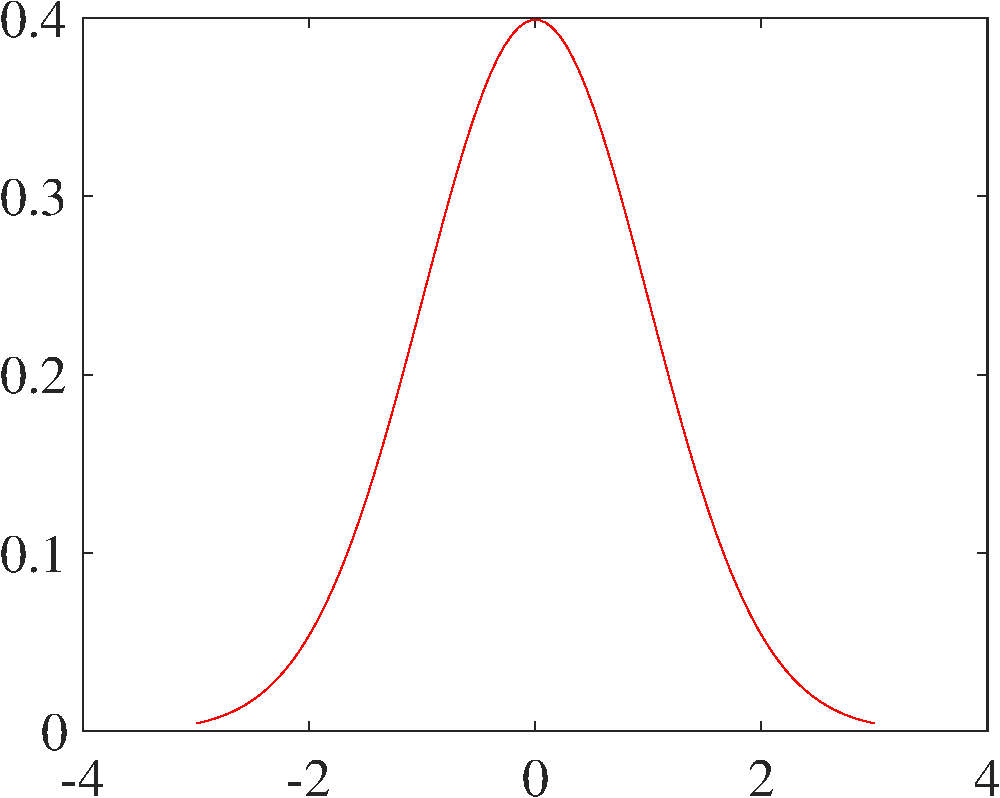
\includegraphics[width=0.5\textwidth]{myGaussian}}
\caption{Plot of the standard Gaussian density.}\label{fig:one}
\end{figure}

Of course in most cases you would probably want to hide the MATLAB
code that was used to generate the figure (although in early versions
of the paper you might want it there for debugging). The histogram in
Figure \ref{fig:two} has the code hidden using the
\texttt{\textbackslash begin\{matlab\} ... \textbackslash
  end\{matlab\}} environment.
\begin{matlab}
%}
a = randn(1000, 1);
b = hist(a, 30);
bar(b);
set(gca, 'fontname', fontName, 'fontsize', fontSize);
print -depsc myHistogram.eps
system('epstopdf myHistogram.eps');
%{
\end{matlab}
\begin{figure}
\centerline{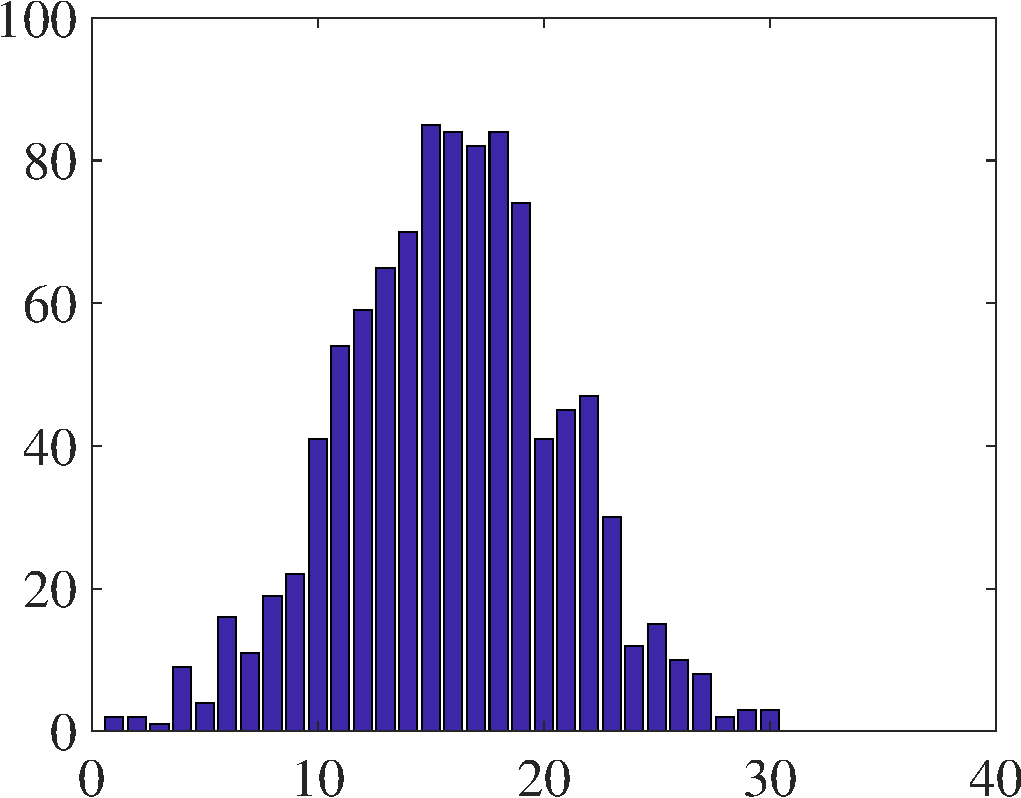
\includegraphics[width=0.5\textwidth]{myHistogram}}
\caption{Histogram of 1000 samples from the standard Gaussian
  density.}\label{fig:two}
\end{figure}

These tricks should allow anyone to recreate your figures if they have
the \LaTeX\ source file.

You could also use the \texttt{listings} package to display your
MATLAB/Octave code to better effect.

You can even use the system to generate tables, or other text to be
included directly in your \LaTeX\ document,
\begin{matlabv}
%}
% Code for generating a table of random numbers.
rows = 3;
cols = 4;
numSigFigs = 3;
resultMatrix = randn(3, 4); % Would normally come from an algorithm.
fid = fopen('results.tex', 'w');
for i = 1:rows
  for j = 1:cols
    fprintf(fid, ['$' num2str(resultMatrix(i, j), numSigFigs) '$']);
    if j < cols
      fprintf(fid, ' & ');
    end
  end
  if i < rows
    fprintf(fid, '\\\\\n');
  end 
end
fclose(fid);
%{
\end{matlabv}

The results file can then be incorporated using \texttt{\textbackslash
  input\{results.tex\}} and placed as in Table \ref{table:one}.
\begin{table}
\caption{A table of random numbers generated in MATLAB/Octave.}\label{table:one}
\begin{center}
\begin{tabular}{c|c|c|c}
$A$ & $B$ & $C$ & $D$ \\
\hline
$0.351$ & $-0.466$ & $-1.57$ & $0.647$\\
$0.122$ & $1.24$ & $0.941$ & $0.462$\\
$-1.03$ & $-1.39$ & $0.605$ & $-0.439$
\end{tabular}
\end{center}
\end{table}

\subsection{Tip}

I like to start my \LaTeX\ files with a series of set up commands from
MATLAB, such as loading in the right path, clearing the memory space,
setting the random seed. That means that you can get consistent
results from running the document. Have a look at the source code to
see it being done for this document.

\subsection{Note for Beamer Users}

If you use the MATweave techniques in your slides using Beamer, you
will have to use the option \texttt{[fragile]} for any frame that
contains the MATLAB environment, as without this option Beamer cannot
handle \texttt{verbatim} or \texttt{comment} environments.

You will need to use MATLAB R14 or higher or Octave 3.2 or higher. Then, to
compile this file under Unix write
\begin{verbatim}
octave --eval source\ myexample.tex
\end{verbatim}
or 
\begin{verbatim}
matlab < myexample.tex
\end{verbatim}
then
\begin{verbatim}
pdflatex myexample
\end{verbatim}

\section{Conclusions}

With a couple of simple tricks, its possible to integrate your MATLAB
and Octave code. This has the advantage of ensuring that what you say
is right beside what you do in your \LaTeX\ source file. The system is
slightly less elegant than the bespoke Sweave system for R, where
plots are automatically incorporated when produced, but it comes with
a lot of flexibility to incorporate the results you want in the final
document.

The aim of MATweave is to make it easier for researchers to produce
\emph{really} reproducible research. Please send comments or
suggestions to the author.

\subsection*{Notes}

The results in this document were generated using MATweave. Code was
run using MATLAB version 9.2 on the architecture
\verb+MACI64+. Experiments were run on 02/09/2017.

\bibliographystyle{plain}
\bibliography{lawrence,other,zbooks}

\end{document}
%} 
% Don't forget to end your MATLAB comment at the end of the file!
